% первая глава

\section{Методы получения трехмерных изображений из двумерных}

В ходе выполнения проекта, главным образом, решается задача преобразования двумерных изображений в трехмерные на мобильных устройствах.

В последние годы заметное место в области преобразования и фильтрации изображений занимает задача преобразования двумерных изображений в трехмерные. На сегодняшний день в мире для этого разработаны различные методики, которые позволяют автоматически создавать так называемые «карты глубины»~\cite{depthMap3} (рисунок ~\ref{fig:s-63}) для двумерных изображений, основываясь на свойствах этого изображение и на некоторых предположениях о характере сцены. 

\begin{figure}[H]
	\centering
	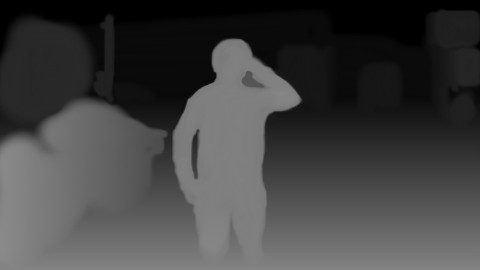
\includegraphics[width=0.7\linewidth]{pics/s-63}
	\caption{карта глубины}
	\label{fig:s-63}
\end{figure} В частности, были проведены исследования следующих методов получения трехмерных изображений из двумерных:

\begin{itemize}
	\item Предположение о том, что изображение имеет линейную перспективу;
	\item Предположение о том, что снимок сделан на открытом пространстве и использование модели рассеяния световых лучей в атмосфере;
	\item Обнаружение теней и восстановление по ним карты глубины;
	\item Обнаружение перекрытий объектов на изображении и используя эту информацию восстановлении карты глубины;
	\item Использование моделей пространственных искажений заданных текстур;
	\item Использование билатеральных симметричных шаблонов;
	\item Использование статистических методов для обучения текстурных шаблонов, на различных расстояниях от объектива и другие методы.
\end{itemize}

Практически все эти методы характеризуются достаточно узким характером сцен, которые могут быть реализованы для преобразования в трехмерное изображение. 

Проведенные предварительные исследования показали, что одним из наиболее перспективных методов преобразования изображений в трехмерные считается метод «дефокусировки», который предполагает, что близкие объекты находятся в фокусе, а более удаленные объекты имеют большее размытие. Используя информацию о размытии той или иной точки на изображении можно предположить о том, насколько далеко она находится от объектива. Используя метод дефокусировки можно построить карту глубины для любой макрофотографии. 

Известные методы получения карты глубины, использующие дефокус удаленных от объектива объектов, основаны на следующей цепочке преобразования изображения~\cite{depthMap1}:

\begin{enumerate} 
	\item Обнаружение краев объектов с использованием фильтра Канни.
	\item Для каждой точки найденного края выполняется оценка расстояния, до нее с использованием гауссовского размытия. Таким образом строится так называемая разреженная карта глубины, которая несет информацию о расстоянии до объектива в некоторых точках изображения. 
	\item Разреженная карта глубины с использованием интерполяции превращается в так называемую «плотную карту глубины», которая уже пригодна для построения трехмерного изображения сцены с любого ракурса. 
\end{enumerate}

Реализация мобильного приложения позволяющего оперативно переводить стандартные фотоизображения в 3D-снимки чрезвычайно актуально и востребовано. С другой стороны, на сегодняшний день имеется определенный научный задел по разработке алгоритмов преобразования 2D -3D. В частности известен ряд различных методик, которые позволяют автоматически создавать «карты глубины» для двумерных изображений, основываясь на свойствах этого изображение, и на некоторых предположениях о характере сцены. Например метод дефокусировки позволяет построить карту глубины фотографии. Вместе с тем информации о программно реализованных в том числе мобильных приложений крайне мало. 

Рассмотренный метод преобразования (см. пункты 1-3) предыдущего раздела страдает двумя существенными недостатками\cite{depthMap2}.

\begin{enumerate}
	\item Разреженная карта глубины получается не всегда гладкой, что приводит к ошибкам последующей интерполяции и, в итоге, к ошибкам в карте глубины. 
	\item Окончательная интерполяция для построения требует больших вычислительных затрат и до последнего времени не имела возможности быть встроенной в мобильные приложения. 
\end{enumerate}

Основываясь на этих двух недостатках существующего метода дефокусировки изображения, требуется провести научное исследование в следующих направлениях:

\begin{enumerate}
	\item Адаптивное сглаживание разреженной карты глубины.  С использованием методов кластеризации краев изображения, в протяженные структуры, глубина точек которых должна подчиняться некоторому закону, а не быть случайной от точки к точке, как в существующем методе. 
	\item Найти способ снижения вычислительных затрат для выполнения двумерной интерполяции при построении плотной карты глубины. 
	\item Нам представляется, что для преобразования двумерного видеоролика в трехмерное представление необходимо разработать методику передачи разреженной карты глубины (с учетом сглаживания) от кадра к кадру. 
\end{enumerate}

Таким образом предлагаемый Проект на сегодняшний день актуален и содержит помимо научной алгоритмической составляющей широкие перспективы коммерциализации.

\section{Технические требования.}

В ходе выполнения проекта будет создана методика количественной оценки достоверности построения карты глубины, которая необходима для корректного преобразования 2D изображения в 3D вид. Эта методика основана на сравнении показаний глубины, полученных в результате работы алгоритмов преобразования 2D –> 3D и достоверных показаний глубины для данной сцены, которые получены в ручном режиме.

Для реализации методики предполагается произвести ручную разметку тестовых цифровых фотографий в количестве не менее 100 штук. Для этого в ручном режиме устанавливаются контрольные точки, с указанием расстояния до них.

Таким образом формируется разреженная карта глубины, с указанием абсолютных значений. Далее, на изображении находится самая дальняя контрольная точка и все расстояния нормируются на расстояние до нее. Таким образом формируется разреженная карта глубины с относительными расстояниями, и, как следствие, (алгоритмически) формируется «эталонная» плотная карта глубины.

Далее, в результате работы различных алгоритмов преобразования изображения из двумерного в трехмерное автоматически вычисляется как разреженная карта глубины для каждого из анализируемых алгоритмов (создаваемого в рамках проекта и конкурирующих аналогов). Далее предполагается вычислять среднеквадратичную ошибку между эталонными значениями для карты глубины и значениями, вычисленными каждым из алгоритмов.

Предполагается, что алгоритм, реализуемый в ходе выполнения проекта даст снижение такой ошибки между вычисленными и эталонными значениями на величину не менее 25\% (ожидаемое значение – порядка 30\%).

Необходимая задача при реализации проекта - адаптация существующего метода преобразования 2D в 3D для использования под управлением операционной системы Android.

В ходе выполнения проекта будут созданы мобильные приложения со следующими характеристиками:

\begin{itemize}
	\item мобильное приложение, функционирующее под управлением операционной системы Android версии не ниже 5.0.
	\item специальных дополнительных требований к аппаратному обеспечению мобильных устройств не предъявляется. Они соответствуют требованиям, накладываемым вышеперечисленными версиями ОС.
	\item мобильные приложения должны функционировать на устройствах с разными размерами экрана от 2.6 до 6 дюймов с разрешениями от 240х320 до 1440х2560 пикселей.
	\item источник данных для конвертирования - файлы в формате jpeg из галереи мобильного устройства или фотография, сделанная штатной фотокамерой мобильного устройства.
	\item мобильные приложения должны обеспечивать конвертацию сделанных фотокамерой изображений при максимальном качестве съемки не менее 10 Мп.
	\item формат данных, в которых сохраняются результаты --- анаглиф файлы (формат jpeg), стерео пара (формат jps), анимированные файлы в формате gif.
	\item ориентировочное время преобразования 2D в 3D не должно превышать 5 секунд.
\end{itemize}

Основные технические параметры, определяющие количественные, качественные характеристики:

\begin{itemize}
\item 3D режим фотосъемки.
\item 3D режим видеосъёмки. 
\item Цифровая стабилизация изображения.
\item Передача файлов в формате Stereo JPEG (*.jps) на внешние устройства. 
\item Отображение файлов в формате Stereo JPEG (*.jps) на мобильном устройстве. 
\item Время преобразования цифровой фотографии в стереоизображение JPEG (*.jps) не превышает 5ти секунд. 
\item Возможность преобразования любой цифровой фотографии из галереи телефона в формат Stereo JPEG (*.jps)
\end{itemize}

\subsection{Технологические требования}

Создаваемое в рамках проекта мобильное приложение должно
функционировать под управлением мобильных операционных систем Android.

\begin{itemize}
	\item Программное обеспечение должно создаваться в строгом соответствии с модульным принципом.
	\item Программное обеспечение должно быть реализовано в виде <<нативных>> приложений для вышеперечисленных операционных систем.
	\item Ожидаемое время преобразования цифровой фотографии в трехмерный вид не должно превышать 5ти секунд. 
\end{itemize}

Технические требования к аппаратному обеспечению мобильного устройства и ограничения, накладываемые на преобразуемые фотографии, будут уточнены в ходе выполнения проекта.

\section{Разработка концепции и архитектуры мобильных приложений, предназначенных для преобразования 2D в 3D.}
В ходе выполнения работы были рассмотрены различные варианты для создания мобильных приложений, предназначенных для преобразования 2D изображений в 3D вид. При этом рассмотрении учитывалось, что результирующие мобильные приложения должны создаваться под операционные системы Android и iOS, а также то, что один из основных результатов работы приложения с точки зрения конечного пользователя – это возможность публикации созданного 3D-изображения в виде анимированного gif-файла в одном или нескольких аккаунтов в социальных сетях пользователя. Соответственно, можно исходить из предположения о том, что для функционирования приложения в любом случае необходим доступ к сети интернет. Максимальная унификация различных составных частей приложения между собой хотя бы на уровне исходных кодов вне зависимости от целевой платформы (Android или iOS) является дополнительным преимуществом при рассмотрении различных вариантов создания мобильных приложений.

Один из наиболее простых с технической точки зрения вариантов реализации решения, позволяющего преобразовывать 2D файлы в 3D вид, является решение, основанное на создании веб-сервиса, который предоставляет минимально необходимый пользовательский интерфейс для загрузки желаемого файла на сервер, преобразования файла на сервере и, как результат, возможность скачать получившийся файл на устройство пользователя и поделиться этим файлом в социальных сетях. При простоте архитектуры у этого решения есть один существенных недостаток – как правило, такие решения менее удобны и функциональны, чем нативные (native) мобильные приложения, разработанные специально под целевую платформу, на которой они будут функционировать. Поэтому на данном этапе от такого подхода было принято решение отказаться.

Если рассматривать варианты создания нативных мобильных приложений, существует несколько возможных вариантов:

\begin{enumerate}
	\item Использовать наиболее популярные средства разработки и языки программирования для каждой из необходимых мобильных платформ. Создать нативное мобильное приложение, реализующее весь необходимый пользовательский интерфейс, набор сервисных функций. Портировать алгоритм преобразования графического файла из 2D в 3D для локального исполнения на мобильном устройстве. Все необходимые преобразования выполнять локально, на мобильном устройстве. Полученный результат преобразования (анимированный gif) загружать в интернет (социальные сети) по мере его готовности на мобильном устройстве.
	\item Использовать наиболее популярные средства разработки и языки программирования для каждой из необходимых мобильных платформ для создания нативных мобильных приложений только для реализации пользовательского интерфейса и набора сервисных функций. Алгоритм преобразования графического файла из 2D в 3D реализуется в виде серверного модуля, соответственно для преобразования выбранного файла и предварительного просмотра полученных результатов необходимо загрузить этот выбранный файл на сервер. Загрузить полученный результат с сервера и поделиться этим результатом в социальных сетях.
	\item Использовать кроссплатформенное средство разработки мобильных решений Xamarin. Это средство одновременно позволяет создавать iOS, Android и Windows Phone приложения. Реализация алгоритма преобразования графического файла из 2D в 3D модифицируется таким образом, что может быть непосредственно интегрирована в Xamarin-проект. В результате получается единое решение, которое на этапе сборки может быть превращено в полнофункциональное нативное приложение для любой из поддерживаемых платформ --- iOS, Android и Windows Phone. Результирующее решение будет преобразовывать графические файлы из 2D в 3D локально на мобильном устройстве, доступ к интернету необходим только для реализации функции «поделиться созданным 3D-файлом в социальных сетях».
	\item Использовать кроссплатформенное средство разработки мобильных решений Xamarin, но только лишь для создания нативных мобильных приложений. реализующих пользовательский интерфейс и набор сервисных функций. Алгоритм преобразования графического файла из 2D в 3D реализуется в виде серверного модуля, соответственно для преобразования выбранного файла и предварительного просмотра полученных результатов необходимо загрузить этот выбранный файл на сервер. Загрузить полученный результат с сервера и поделиться этим результатом в социальных сетях.
\end{enumerate}

Перед тем, как рассмотреть каждый из приведенных выше вариантов по отдельности, следует отметить, что существующая на сегодняшний день реализация алгоритма преобразования изображений из 2D в 3D вид реализована на языке С++, сборка осуществляется с использованием Microsoft Visual Studio, соответствующее решение имеет существенную зависимость от OpenCV (Open Source Computer Vision Library – это программная библиотека с открытым исходным кодом, реализующая базовые алгоритмы компьютерного зрения, обработки изображений и численных алгоритмов общего назначения. Реализована на C/C++).

Возвращаемся к вышеперечисленным вариантам.

Для варианта №1 для операционной системы Android необходимо:

С использованием Android Studio на языке программирования Java реализовать необходимый пользовательский интерфейс, а также весь необходимый набор сервисных функций. Необходимо адаптировать реализацию алгоритма преобразования графического файла из 2D в 3D для использования под управлением операционной системы Android (реализация на С++). Далее, с использованием механизма The Android Native Development Kit (NDK) необходимо обеспечить вызов кода, написанного на языке С++ из «классического» Android-приложения. 

Для разработки приложений для iOS основным средством разработки является Objective-C. Проведенные предварительные исследования показали, что адаптировать реализацию алгоритма преобразования графического файла из 2D в 3D для использования под управлением операционной системы iOS с разумными усилиями не представляется возможным. Соответственно, вариант №1 является неприемлемым для реализации решения для операционной системы iOS.

Для реализации варианта №2 необходимо:

С использованием наиболее популярных средств разработки и языков программирования для каждой из необходимых мобильных платформ (Java для Android и Objective С для iOS) необходимо создать нативные мобильных приложений для реализации пользовательского интерфейса и набора сервисных функций. Эта задача, в целом, является типовой и принципиальных сложностей не вызывает. Алгоритм преобразования графического файла из 2D в 3D следует реализовать в виде серверного модуля, например, для использования под управлением операционной системы Ubuntu. Это обусловлено тем, что Unix-подобные операционные системы имеют существенно более широкое распространение в Web-серверном окружении, чем Windows-сервера. Основная сложность данной задачи – в сборке и корректном использовании OpenCV библиотеки под Linux, однако аналогичная задача сравнительно недавно была решена коллегами для реализации демонстрационного видеоплеера для использования под операционной системой Ubuntu.

Для реализации варианта №3 необходимо адаптировать алгоритм преобразования графического файла из 2D в 3D таким образом, чтобы он мог быть непосредственно интегрирован в Xamarin-проект (разработка на языке программирования С\#). Проведенные предварительные исследования показали, что реализовать подобный функционал за разумное время с разумными усилиями не представляется возможным.

Вариант №4 основывается на разработке унифицированного решения для всех поддерживаемых мобильных платформ (iOS, Android и Windows Phone) для реализации пользовательского интерфейса и сервисных функций на языке программирования С\#. В части алгоритма преобразования графического файла из 2D в 3D этот вариант полностью аналогичен (точнее даже унифицирован) варианту №2 – должен быть реализован серверный модуль, например, для использования под управлением операционной системы Ubuntu для реализации этого преобразования. И, соответственно, с помощью реализованных на С\# функций выбирается файл для преобразования, отправляется на сервер, там преобразовывается, скачивается обратно для предварительного просмотра полученных результатов, а далее реализуется возможность поделиться полученным результатом в социальных сетях.

На основе проведенного исследования моно сделать следующий вывод. С точки зрения скорости, легкости и качества реализации наиболее перспективными являются варианты №2 и №4. Однако, вариант №4, в силу кроссплатформенности, унифицированности решения для всех поддерживаемых мобильных платформ является более предпочтительным. Соответственно, на реализации этого варианта и будут сосредоточены усилия на самом первом этапе развития проекта. 

Очевидным недостатком подобного решения является существенная его зависимость от скорости и надежности мобильного интернета, а также от доступности конечному пользователю оплаченного траффика. Для обхода этих ограничений предполагается исследовать возможность создания для пользователей ОС Android «самодостаточного» мобильного приложения (вариант №1), которое все необходимые действия, связанные с преобразованием файлов производит непосредственно на мобильном устройстве. Хочется надеяться, что необходимая для этого адаптация алгоритма преобразования графического файла из 2D в 3D для использования под управлением операционной системы Android (после создания реализации этого алгоритма по Ubuntu, основная проблема – возможность использования OpenCV под соответствующую платформу – должна решаться аналогичным образом) не доставит много хлопот.

\section{Анализ существующих продуктов со схожим функционалом}
Одной из задач при создании мобильного приложения для преобразования 2D фотографий в 3D вид, является разработка пользовательского интерфейса.

Для достижения этой задачи были проанализированы аналогичные приложения, которые очень популярны на сегодняшний день: Prisma, Pixlr, Candy Camera.

В первую очередь, целью сравнения являлся анализ особенностей пользовательского интерфейса этих приложений. Это обусловлено тем, что, во многом, схема функционирования приложения, которое планируется создать в ходе выполнения проекта, аналогична схеме работы этих приложений. А именно: пользователь делает фотографию при помощи штатной камеры своего смартфона или загружает уже существующее изображение из галереи, отправляет изображение на обработку, просматривает результат и, если результат ему нравится, сохраняет или отправляет получившееся изображение в одну или несколько социальных сетей.

Таким образом можно выделить 4 основных окна приложения:
\begin{enumerate}
	\item Режим камеры, делаем фотографию.
	\item Окно выбора фотографии из галереи.
	\item Окно применения фильтра, смотрим готовый результат.
	\item Окно выбора действий с получившейся фотографией.
\end{enumerate}

\subsection{Prisma}
Проанализировав пользовательский интерфейс первого приложения Prisma (рисунок~\ref{fig:prismaCam}), в режиме камера увидели заметные отличия - это наличие статус бара и возможность переключения между камерой, лентой и профилем в верхней части экрана или свайпом, движением пальца по экрану телефона влево и вправо. Все кнопки расположены удобно и их назначения интуитивно понятны. В галереи показаны все изображения, имеющиеся в смартфоне (рисунок ~\ref{fig:prismaGal}). После применения фильтра есть возможность обрезать фото в нужном соотношении (рисунок ~\ref{fig:prismaProp}).

\begin{figure}[H]
	\centering
	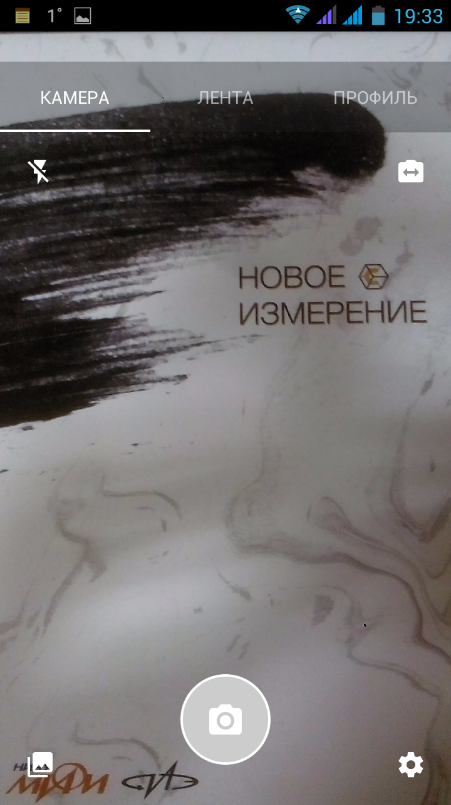
\includegraphics[width=0.3\linewidth]{pics/prismaCam}
	%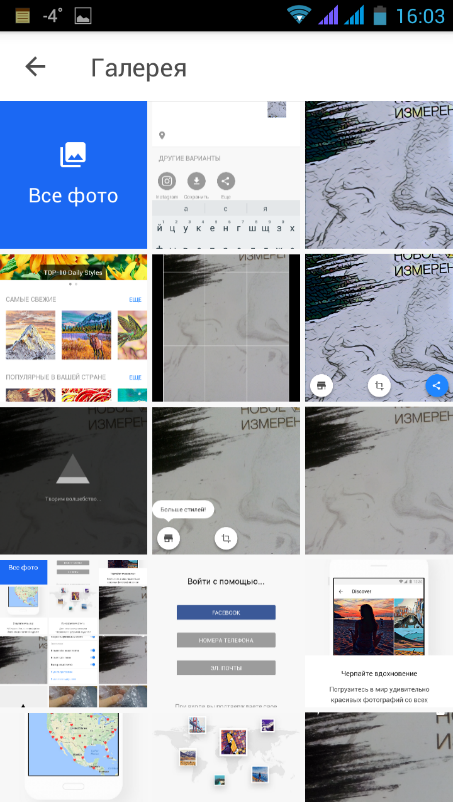
\includegraphics[width=0.3\linewidth]{pics/prismaGal}
	%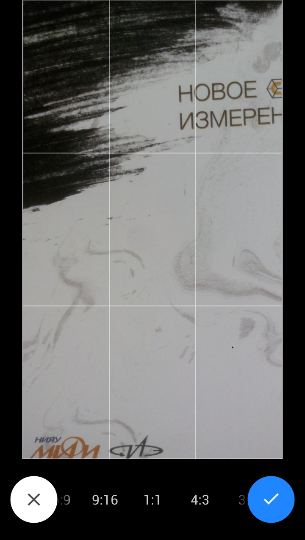
\includegraphics[width=0.3\linewidth]{pics/prismaProp}
	\caption{Prisma, окно с камерой}
	\label{fig:prismaCam}
	\label{fig:prismaGal}
	\label{fig:prismaProp}
\end{figure}

\begin{figure}[H]
	\centering
	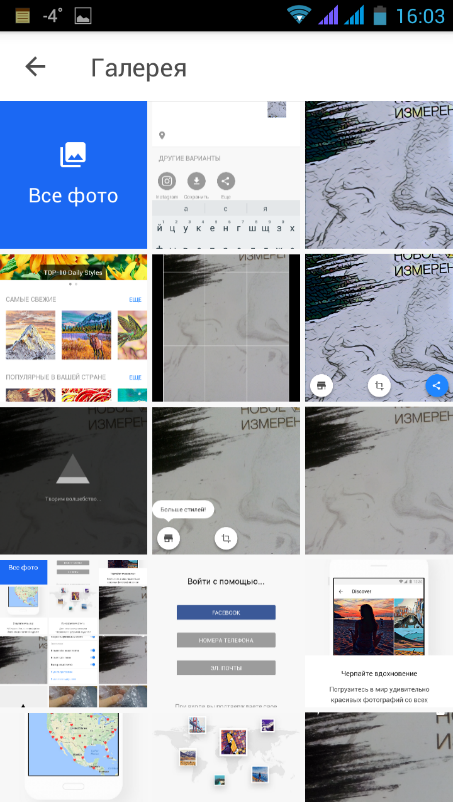
\includegraphics[width=0.3\linewidth]{pics/prismaGal}
	\caption{Prisma, окно с галереей}
	\label{fig:prismaGal}
\end{figure}

\begin{figure}[H]
	\centering
	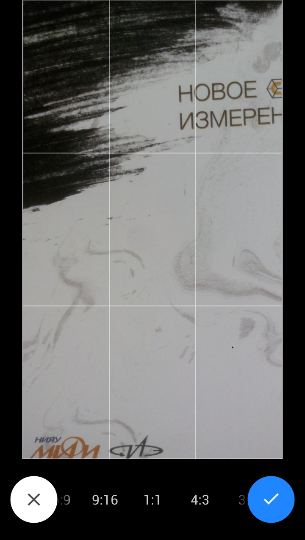
\includegraphics[width=0.3\linewidth]{pics/prismaProp}
	\caption{Prisma, окно выбора пропорции для изображения}
	\label{fig:prismaProp}
\end{figure}

\subsection{Candy Camera}
Проанализировав пользовательский интерфейс приложения Candy Camera (рисунок~\ref{fig:candyCam}), в режиме камеры видим большое количество кнопок, не все их назначения понятны с первого раза. Фильтры и соотношения фотографии применяются сразу в режиме камеры. Заметное отличие заключается в том, что, сделав фотографию есть 3 секунды чтобы выбрать кнопку поделиться с друзьями или удалить фото (рисунок~\ref{fig:candyGal}). Не выбрав ничего продолжается режим фотографирования. После можно вернуться к сделанным фотографиям через галерею, потом применить фильтр и поделиться изображением в социальных сетях (рисунок~\ref{fig:candyPod}). В галереи все изображения рассортированы по дням, в отдельных блоках.

\begin{figure}[H]
	\centering
	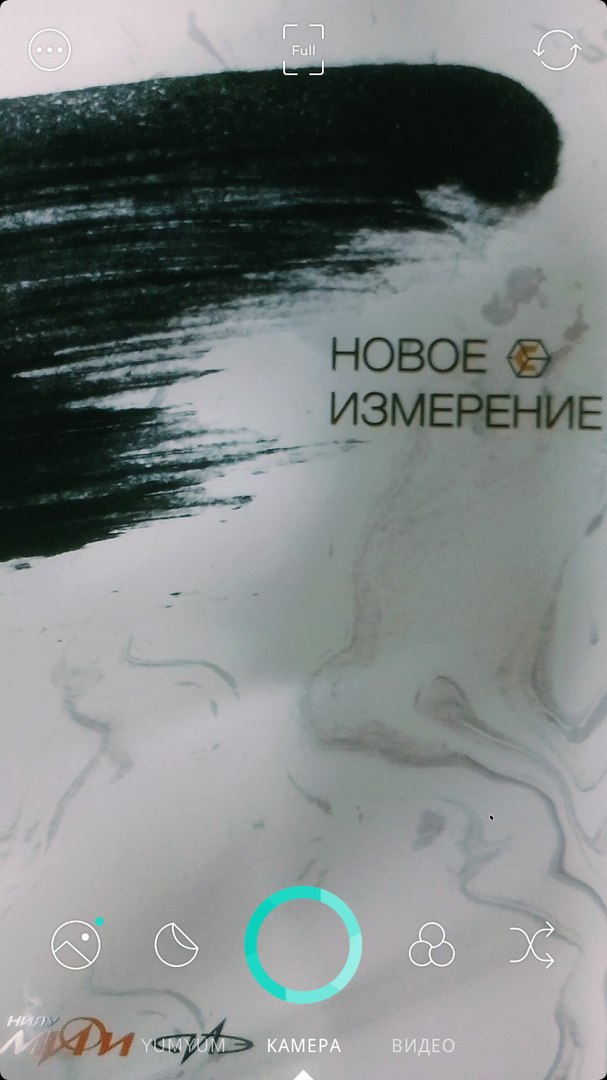
\includegraphics[width=0.3\linewidth]{pics/candyCam}
	\caption{Candy Camera, окно с камерой}
	\label{fig:candyCam}
\end{figure}

\begin{figure}[H]
	\centering
	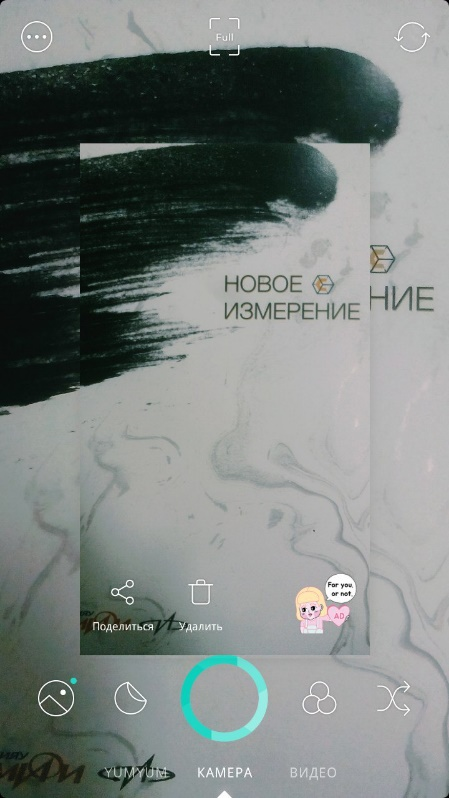
\includegraphics[width=0.3\linewidth]{pics/candyGal}
	\caption{Candy Camera, окно с просмотром фото}
	\label{fig:candyGal}
\end{figure}

\begin{figure}[H]
	\centering
	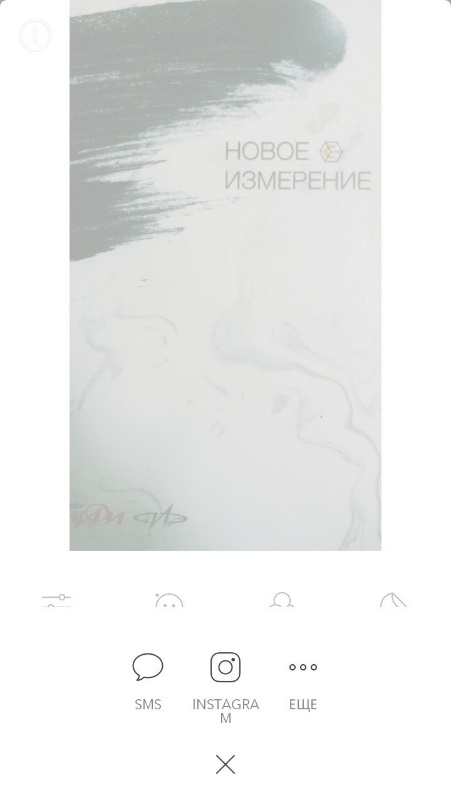
\includegraphics[width=0.3\linewidth]{pics/candyPod}
	\caption{Candy Camera, окно выбора с кем поделиться изображением}
	\label{fig:candyPod}
\end{figure}

\subsection{Pixlr}
Проанализировав пользовательский интерфейс приложения Pixlr (рисунок~\ref{fig:pixlrMenu}), основное различие с предыдущими приложениями это наличие главного меню, которое открывается при запуске программы. В меню можно выбрать дальнейшее действие, открыть камеру и сделать фотографию или открыть галерею и выбрать картинку из имеющихся изображений. Из режима камеры нельзя перейти в галерею (рисунок~\ref{fig:pixlrCam}). Имеются кнопки с фильтрами, которые применяются сразу. Сделав фотографию, мы оцениваем ее и решаем сделать новое фото или продолжить редактировать. Галерея открывается с помощью стандартного просмотрщика галереи этого телефона. Применив фильтр, Pixlr предлагает разместить фото в разных социальных сетях, сохранить изображение или выбрать дополнительные действия с картинкой (рисунок~\ref{fig:pixlrPod}). При сохранении можно выбрать разрешение, формат JPEG или PNG и качество изображения, после сохранения остается возможность поделиться этой фотографией в социальных сетях.

\begin{figure}[H]
	\centering
	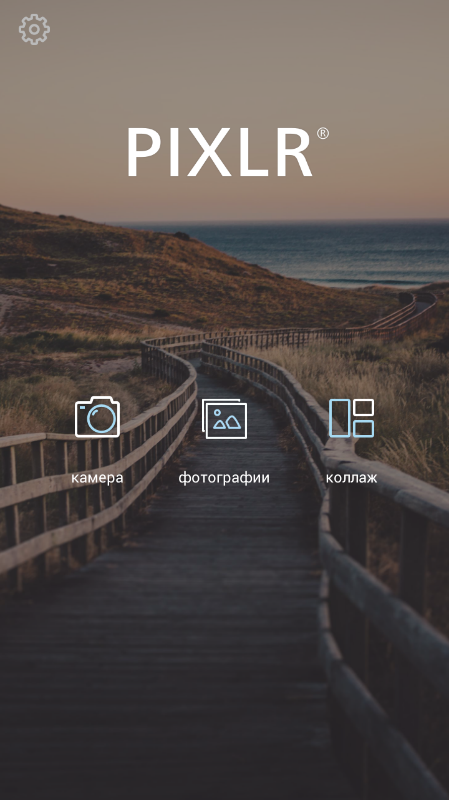
\includegraphics[width=0.3\linewidth]{pics/pixlrMenu}
	\caption{Pixlr, главное меню}
	\label{fig:pixlrMenu}
\end{figure}

\begin{figure}[H]
	\centering
	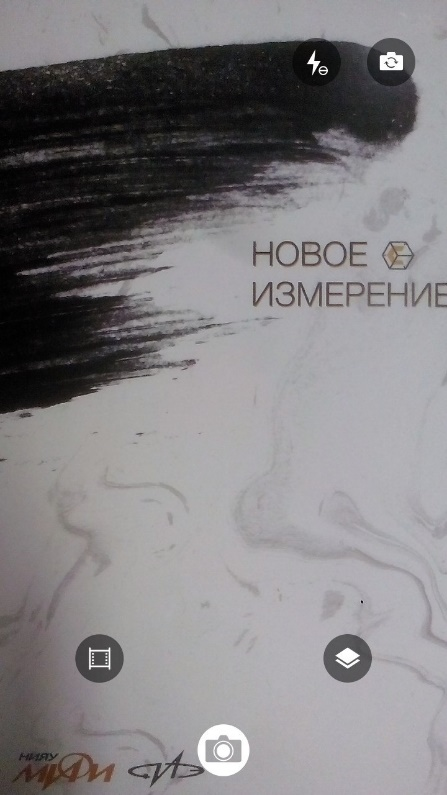
\includegraphics[width=0.3\linewidth]{pics/pixlrCam}
	\caption{Pixlr, окно с камерой}
	\label{fig:pixlrCam}
\end{figure}

\begin{figure}[H]
	\centering
	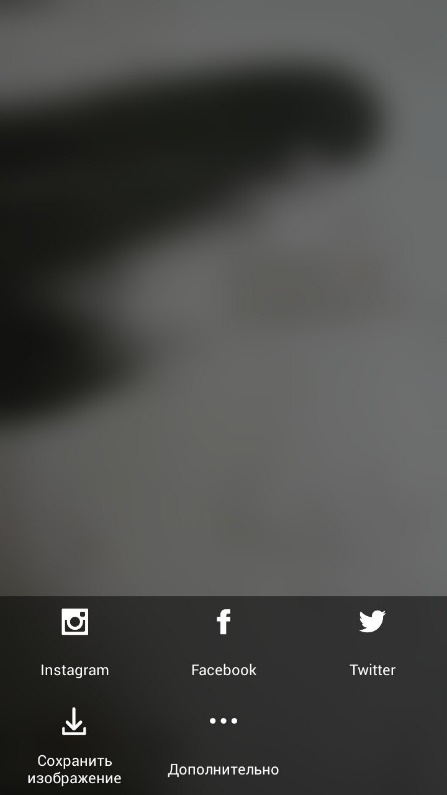
\includegraphics[width=0.3\linewidth]{pics/pixlrPod}
	\caption{Pixlr, окно выбора с кем поделиться изображением}
	\label{fig:pixlrPod}
\end{figure}

\subsection{Анализ интерфейса}
Сравнив данные приложения, увидели общие черты, в режиме камеры имеются кнопки переключения режима фотовспышки и переключение между основной и фронтальной камерами. Есть возможность выбора соотношений, пропорций фотографии. Везде есть возможность поделиться фотографией в Instagram.

У Pixlr есть отличительная черта, это наличие главного меню и отсутствие собственного пользовательского интерфейса галереи. У Prisma, интерфейс галереи реализован лучше чем у Candy Camera. У Pixlr и Candy Camera есть удобная возможность просматривать фильтр в живую, еще не сделав фотографии. В режиме камеры у Pixlr и Prisma, кнопки расположены и выглядят более удобно чем у Candy Camera. Окно выбора действия с отредактированным изображением (сохранить или поделиться фотографией в социальных сетях) у Pixlr реализовано лучше.

Считаю, что необходимый набор функций программы должен включать: выбор фотографии из стандартной галереи, режим камеры, обработка изображения, просмотр результата, возможность сохранить, поделиться фотографией в социальных сетях и дополнительные возможности передачи картинки.

Необходимый набор элементов пользовательского интерфейса камеры должен включать: переключение режимов фотовспышки, переключение главной и фронтальной камеры, кнопку настроек, переход к выбору фотографии из галереи.

Мы планируем сделать приложение следующим образом, при включении откроется камера (рисунок~\ref{fig:cam}), сделав фотографию пользователю предстоит оценить получившуюся фотографию и если нравится, то перейти к редактированию изображения, иначе сделать новое фото (рисунок~\ref{fig:foto}). Сделав удовлетворяющую фотографию или выбрав нужную из галереи, происходит обработка изображения, и пользователь может просмотреть получившуюся картинку. Тут же есть возможность вернуться к камере, обрезать или продолжить. Выбрав продолжить, появляется окно с выбором дальнейших действий с данной фотографией, запостить фото в социальных сетях на выбор, сохранить изображение в пользовательском качестве или дополнительные способы передачи картинки (рисунок~\ref{fig:pod}).

\begin{figure}[H]
	\centering
	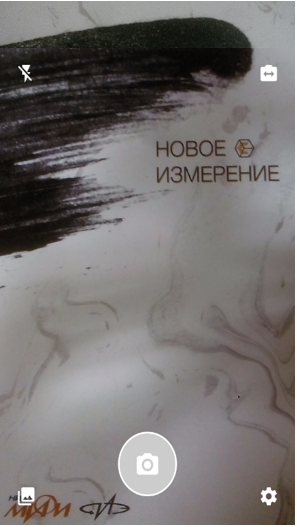
\includegraphics[width=0.3\linewidth]{pics/cam}
	\caption{Окно с камерой}
	\label{fig:cam}
\end{figure}

\begin{figure}[H]
	\centering
	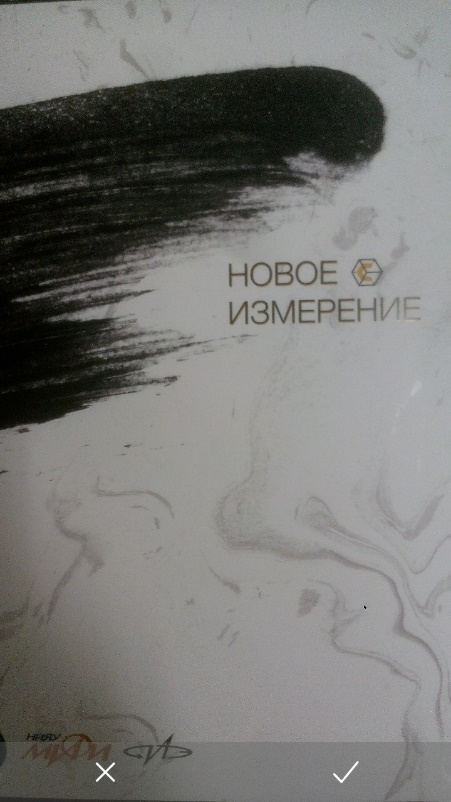
\includegraphics[width=0.3\linewidth]{pics/foto}
	\caption{Окно с просмотром фото}
	\label{fig:foto}
\end{figure}

\begin{figure}[H]
	\centering
	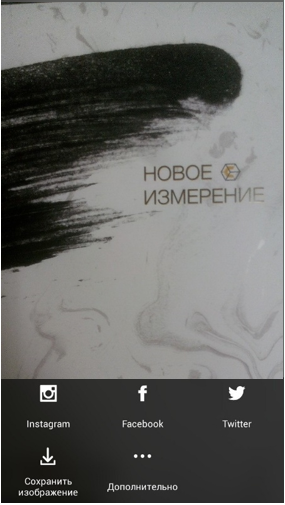
\includegraphics[width=0.3\linewidth]{pics/pod}
	\caption{Окно выбора с кем поделиться изображением}
	\label{fig:pod}
\end{figure}

При создании пользовательского интерфейса приложения были проанализированы современные, с аналогичным функционалом мобильные приложения в целом. Был сделан акцент на необходимости создания современного, функционального и не перегруженного пользовательского интерфейса. В результате проведенного анализа был создан пользовательский интерфейс мобильного приложения для преобразования 2D фотографий в 3D вид.

